\chapter{A metodologia alkalmazása}

\section{Termékfejlesztési folyamatok vizsgálata}
\subsection{Észlelt hibák biztonsági vizsgálata}

Lsd: Flaw remediation (ALC\_FLR)

\subsection{Fejlesztési- és karbantartási folyamatok}
\subsubsection{Fejlesztési folyamat}
Jelenleg az alábbi állomások vannak egy \emph{feature request} életében:
\begin{description}
    \item[To do] {Jelentése}
    \item[To do] {Jelentése}
    \item[To do] {Jelentése}
    \item[To do] {Jelentése}
    \item[To do] {Jelentése}
\end{description}

\subsubsection{Karbantartási folyamatok}

\subsubsection{Szigorítások a folyamatokon}

A feladatok száma elérte már azt a szintet, hogy nem tudjuk fejben megbízhatóan követni őket, ezért
a jegyek kezelésére bevezettük a JIRA-t, így a fejlesztő tudja frissíteni dolgozott jegy állapotát.
Sajnos tetszőleges átmenet megengedett két állapot között, így felmerülnek olyan, minőségbiztosítási
szempontból aggályos kiskapuk,

Ezért első közelítésben korlátozni kell a lehetséges átmeneteket az alábbiakra.

Belátható, hogy ez nem elégséges, ezzel csak annyit értünk el, hogy a rosszindulatú fejlesztőnek
kicsit több időbe telik a szándékolt változtatás, ezért az alábbi előfeltételek és automatizmusok
szükségesek az átmenetek végrehajtásához.

Ezek a szigorítások elégségesnek bizonyulnak egy átlagos jogkörrel rendelkező fejlesztő
rosszindulatú jegykezelésének megfékezésére, azok ellen hatástalan, akiknek rendszerszintű
jogosultsága van a JIRA felett, de ezen emberek száma már lényegesen kevesebb.

\subsection{Configuration Management}
A \emph{Configuration Management} (továbbiakban: CM) egy olyan rendszer, amely arra hivatott,
hogy azokat a változtatásokat nyomon tudja követni, amelyek hatással lehetnek a vizsgált termékre.
Amennyiben csak jól meghatározott, autorizált változtatásokat engedélyezünk, biztosíthatjuk a
termékünk integritását.
Természetesen mielőtt egyáltalán bevezetnénk a \emph{CM}-et, feltétlenül szükséges meghatározni
annak hatókörét. Erre szolgál a \emph{ALC\_CMS} szekció.

\subsubsection{Configuration Management Scope}
\begin{itemize}
    \item{ALC\_CMS.1}
    \item{ALC\_CMS.2}
    \item{ALC\_CMS.3}
    \item{ALC\_CMS.4}
    \item{ALC\_CMS.5}
\end{itemize}

\pagebreak[0]
\subsubsection{Configuration Management - termék verziózása}
\subsubsection{Az első szint követelményei}
\begin{quote}
    \begin{description}
        \item[ALC\_CMC.1.1D]{The developer shall provide the TOE and a reference for the TOE.}
        \item[ALC\_CMC.1.1C]{The TOE shall be labelled with its unique reference.}
    \end{description}
\end{quote}

Az EAL1 szint elérése ennél az alosztálynál egy egészen egyszerű feladatnak tűnik, hiszen csupán
annyi a feladat, hogy a termék egy adott állapotát egy egyedi cimkével ellássuk, és mivel a
verziószám készítése manapság elterjedt, ezért adódik, hogy legyen ez az egyedi cimkénk.

Sajnos ez csak addig ennyire egyszerű, amíg nem jutunk el a kiadás létrehozásáig:
vannak olyan teszteseteink (továbbiakban: \emph{Release teszt}),
amelyek futtatása költséges, és/vagy különleges helyeken kell azt
futtatni. Ezt a problémát úgy oldottuk fel, a létrehozott kiadáson hajtjuk végre ezeket.
Amennyiben anomáliát észlelünk, a javítástól újraindítjuk a termékfejlesztés folyamatát,
és \emph{a cimkét átmozgatjuk a javított állapotra}, amellyel azonnal megsérthetjük az egyedi
cimkét, ha az átmozgatás nem mindenütt történik meg.

Adódik a javaslat is, hogy külön jelöljük azokat a verziókat, amelyek eljutottak a Release tesztig,
például a széles körben használt \emph{sorszámozott Release Candidate}, röviden \emph{rc}
szuffixszel.
Alternatív módszerek lehetnek az alábbiak:
\begin{itemize}
    \item \emph{git describe} használata: \\
        Például: \emph{syslog-ng-3.7.2-834-gdb3795a}, amely az alábbi formátumnak felel meg: \\
        \emph{<commit-tól a szülők felé lépdelve az első elérhető tag>-<az elért tagtől hány commit
            történt a paraméterben kapott commit-ig>-<verziókezelőt leíró karakter><paraméterben
        átadott commit commitid-ja>}
\end{itemize}

\pagebreak[0]
\subsubsection{Configuration Management - CM rendszer használata}
\subsubsection{Mi változott az előző szinthez képest?}

\begin{quote}
    \begin{description}
        \item[ALC\_CMC.2.2D]{\emph{The developer shall provide the CM documentation.}}
        \item[ALC\_CMC.2.3D]{\emph{The developer shall use a CM system.}}
        \item[ALC\_CMC.2.2C]{\emph{The CM documentation shall describe the method used to uniquely
            identify the configuration items.}}
        \item[ALC\_CMC.2.3C]{\emph{The CM system shall uniquely identify all configuration items.}}
    \end{description}
\end{quote}
Belátható, hogy a \emph{git} verziókezelő rendszer széleskörű használata kezdetben megfelelő
lehet CM rendszernek is.

\pagebreak[1]
\subsubsection{Configuration Management - Autorizáció}
\subsubsection{Mi változott az előző szinthez képest?}
\begin{quote}
    \begin{description}
        \item[ALC\_CMC.3.4C]{\emph{The CM system shall provide measures such that only authorised
            changes are made to the configuration items.}}
        \item[ALC\_CMC.3.5C]{\emph{The CM documentation shall include a CM plan.}}
        \item[ALC\_CMC.3.6C]{\emph{The CM plan shall describe how the CM system is used for the
            development of the TOE.}}
        \item[ALC\_CMC.3.7C]{\emph{The evidence shall demonstrate that all configuration items are
            being maintained under the CM system.}}
        \item[ALC\_CMC.3.8C]{\emph{The evidence shall demonstrate that the CM system is being
            operated in accordance with the CM plan.}}
    \end{description}
\end{quote}

Ez az a pont, ahol a CM rendszer használata értelmet nyerhet, hiszen pont azzal a szándékkal
vezetjük be, hogy csak az autorizált változtatásokat engedélyezze.

Az előző pontban beláttuk a \emph{git} használatának előnyét, és a \emph{git}-et elsődlegesen
forráskódok kezelésére használják, ezért visszavezethetjük a problémánkat oda, hogy hogyan
\emph{szokás} a forráskód módosításainál eldönteni, hogy az autorizált-e.
Észrevehetjük, hogy a nyílt, közösség által fejleszett projektek ezt meg tudják
úgy oldani, hogy:
\begin{itemize}
    \item{csak olyan változtatások kerülhetnek be a kódbázisba, amelyet egy szűkebb csoport elfogad,}
    \item{továbbá megmarad a lehetőség arra, hogy akárki képes legyen kontributálni.}
\end{itemize}

Azért képesek erre, az úgynevezett \emph{Forking Workflow}-t használják a fejlesztésre, amely röviden
az alábbi lépésekből áll:
\begin{enumerate}
    \item{Létrejön egy ún. \emph{blessed repository}, amely a forráskód referenciaváltozatát
        tartalmazza.}
    \item{Az egyes fejlesztők leklónozzák ezt a \emph{repository}-t sajátként.}
    \item{A fejlesztő a saját \emph{repository}-jában elkészíti a módosításait.}
    \item{Valamilyen módon értesíti a \emph{blessed repository} tulajdonosát
        (nevezzük ezt a személyt \emph{integrátornak}) az elkészített változtatásokról.}
    \item{Az integrátor elfogadja, vagy elveti a javasolt változtatásokat.}
\end{enumerate}

\begin{figure}[h]
    \centering
    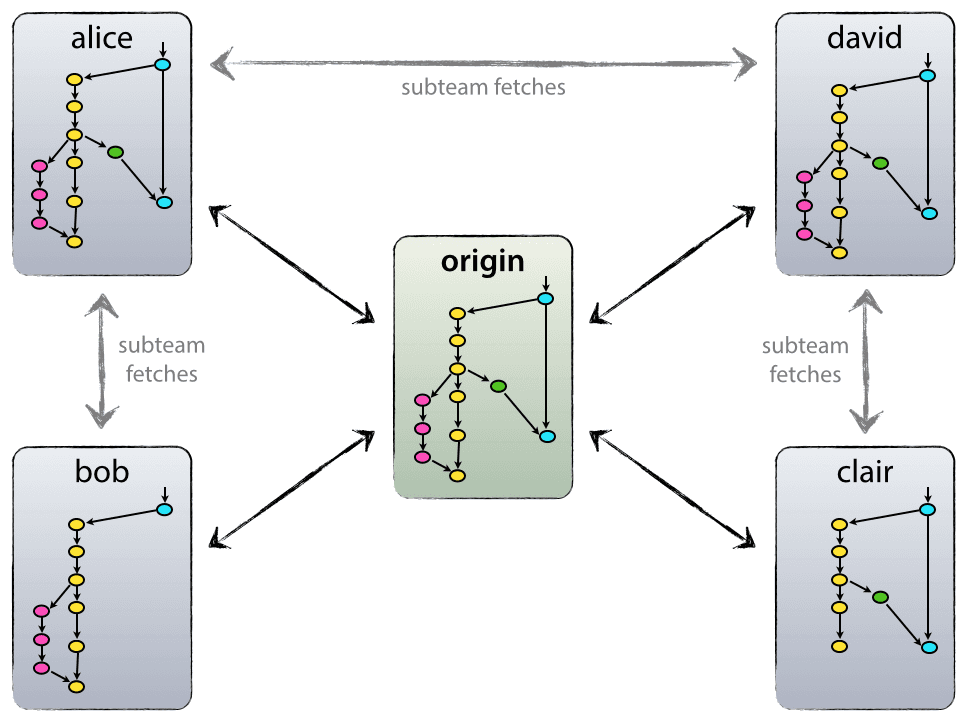
\includegraphics[width=\textwidth, height=0.25\textheight, keepaspectratio]{figures/forkingworkflow.png}
\end{figure}
\FloatBarrier

Természetesen ahhoz, hogy ez működjön, meg kell tiltani a \emph{blessed repository} írását a
többi fejlesztő által, vagy legalábbis csak kivételes esetekben szabad ezeket engedélyezni.

A \emph{syslog-ng}-nél a közösség által fejlesztett változatban már korábban igazodni kellett
ehhez a munkafolyamathoz, a kereskedelmi célú változatában ezt a gondolkodásmódot még erősíteni
szükséges, mivel általában a módosítások integrálásának kérelme (továbbiakban: \emph{pull/merge request})
meg szokott történni, de ez a \emph{blessed repository} egyik ágának a másikára szokott történni,
azaz semmi sem garantálja, hogy egy rosszindulatú fejlesztő képtelen legyen tetszőleges módosítást
végrehajtani a kódbázison.

\pagebreak[1]
\subsubsection{Configuration Management - Production support, acceptance procedures, automation}
\subsubsection{Mi változott az előző szinthez képest?}
\begin{quote}
    \begin{description}
        \item[ALC\_CMC.4.4C]{The CM system shall provide \emph{automated} measures such that only
            authorised changes are made to the configuration items.}
        \item[ALC\_CMC.4.5C]{\emph{The CM system shall support the production of the TOE by
            automated means.}}
        \item[ALC\_CMC.4.8C]{\emph{The CM plan shall describe the procedures used to accept
            modified or newly created configuration items as part of the TOE.}}
    \end{description}
\end{quote}
Azaz ez a szekció a magasabb szintű automatizálás megvalósítására hivatott, mivel az alapfeltételezés
az, hogy az emberi tényező megbízhatósága lényegesen alacsonyabb lehet egy megegyező munkát végző
géppel, főként az amúgy könnyedén automatizálható feladatoknál.
Mint ahogy az a követelményekből látszik, a \emph{Common Criteria} csak az autorizált változtatások
bekerülését szabályozná automatikusan, viszont ha az \emph{4.8C}-ben említett pontot kellőképpen
formálisan írjuk le, akkor abból könnyedén programkód készülhet, és végsősoron az ellenőrzések egy
részhalmazát automatikusan is ellenőrizhetjük.

A \emph{syslog-ng} közösség által fejlesztett változatánál a legnagyobb elmaradás az elfogadás
szükséges feltételeinek dokumentálása, és az automatizálható ellenőrzések automatizálása.

Ennél a pontnál felmerült egy olyan eszköz létrehozása, 

Van az ellenőrzéseknek egy olyan fajtája, amelyeket csak az újonnan beérkező kódra szeretnénk
alkalmazni. Tipikus példa erre a kódstílus egységesítése: ha ezt a kódbázisra azonnal alkalmazni
szeretnénk, akkor az túl nagy különbséget eredményezne. A stílus leírójának változásának alkalmazása
ugyanúgy nagy különbséget eredményezne. Például ha a jelenlegi \emph{master} ágon szeretném az
összes \emph{C} nyelven írt forrásfájlt formázni, akkor az önmagában egy $16375$ sor hozzáadásával
és $15982$ sor törlését eredményezi.
Belátható, hogy ennek szakmai lektorálása (gyakrabban használt kifejezéssel \emph{(peer) review}-ja)
nehézkes annak mérete miatt, a lektorálatlan kód pedig lehet, hogy kártékony módosításokat tartalmaz.
A kártékony módosítások kiszűrése a legfontosabb feladata a lektornak, hiszen a \emph{syslog-ng}
tipikusan \emph{root} felhasználóként fut.


\subsubsection{Configuration Management - fejlett támogatás}
\subsubsection{Mi változott az előző szinthez képest?}
\begin{quote}
    \begin{description}
        \item[ALC\_CMC.5.3C]{The CM documentation shall justify that the acceptance procedures
            provide for an adequate and appropriate review of changes to all configuration items.}
        \item[ALC\_CMC.5.7C]{The CM system shall ensure that the person responsible for accepting a
            configuration item into CM is not the person who developed it.}
        \item[ALC\_CMC.5.8C]{The CM system shall identify the configuration items that comprise the
            TSF.}
        \item[ALC\_CMC.5.9C]{The CM system shall support the audit of all changes to the TOE by
            automated means, including the originator, date, and time in the audit trail.}
        \item[ALC\_CMC.5.10C]{The CM system shall provide an automated means to identify all other
            configuration items that are affected by the change of a given configuration item.}
        \item[ALC\_CMC.5.11C]{The CM system shall be able to identify the version of the
            implementation representation from which the TOE is generated.}
    \end{description}
\end{quote}

\pagebreak[2]
\subsection{Delivery}

Ennek a szekciónak a célja olyan intézkedések/követelmények megfogalmazása, amelyek
biztosítják, hogy a felhasználóhoz biztonságosan jut el a termékünk.

\section{Development Security}

